\section{What counts as evidence}
\label{sec:evidence}

A representation-level claim is read here in three steps. The first separates evidence that a concept is
encoded in a representation from evidence that the model uses it (\S\ref{sec:two-questions}), a
distinction that fixes what any single measurement can support. The second grades interventional
evidence on three rungs of increasing strength (\S\ref{sec:causal-claims}) and states the estimand that
each method family reports (\S\ref{sec:formal}). The third names the properties against which an
artefact is validated, and how often this corpus reports them (\S\ref{sec:eval-what}).
Fig.~\ref{fig:families} draws the resulting ladder, from observation to concept-specific causal
contribution.

\subsection{Two questions}
\label{sec:two-questions}

The first question, \emph{what does the representation
encode?}, is answered observationally: by fitting $g$, computing similarities, decomposing $z_\lambda$ or
locating information along the path. The second, \emph{what does the model use?}, requires an
intervention on $z_\lambda$ and an observed change in $B$. This distinction follows the first two levels
of the causal hierarchy~\cite{bareinboim2022pearl}. The two questions are not interchangeable. A concept can be linearly
decodable from a representation that the output never uses, so probing accuracy overstates use, as
control tasks, amnesic probing, concept erasure and direct tests of task relevance established for
language
models~\cite{hewitt2019designing,elazar2020amnesic,ravfogel2020null,belrose2023leace,ravichander2021probing,ivanova2021probing}.
The converse error also exists: an uncontrolled intervention that changes behaviour shows that the
output is sensitive to the representation, not that the direction means what it was named. The
taxonomy of \S\ref{sec:taxonomy} tags the two kinds of evidence apart.

A medical instance makes the gap concrete. Frozen CT embeddings from an encoder trained without
demographic labels decode patient sex at AUROC 0.998~\cite{zheng2024demographic}, which establishes that
sex is available to any readout placed on those features. It does not establish that a model built on
them relies on sex when it reports a finding: that requires changing the representation that carries
sex, holding the rest of the computation fixed, and measuring a pre-specified end-point.
\S\ref{sec:decoding} reports the two medical studies that attempt such a test and
\S\ref{sec:intervention} what their controls can and cannot establish.

\subsection{Three causal claims}
\label{sec:causal-claims}

An intervention supports one of three claims of increasing strength, and the rung it reaches is set by
its control rather than by the size of its effect; \S\ref{sec:formal} gives the estimand behind each.
\emph{Causal sensitivity} means that the output changes when $z_\lambda$ is changed; any intervention
whose effect exceeds its uncertainty over inputs establishes it. \emph{Direction-selective sensitivity}
means that the effect of $v_c$ exceeds that of matched controls. \emph{Concept-specific causal
contribution} means that the effect is attributable to the model's representation of $c$ rather than to
a correlated direction. Agreement among independently constructed directions, a correlated-concept hard
negative and an intervention that stays within the empirical activation distribution are necessary for
the third claim, but they do not identify the contribution; identification takes a mediation
design~\cite{pearl2001direct,imai2010mediation}, a causal-concept effect estimated under an
intervention on the concept itself~\cite{goyal2019cace}, or a causal-abstraction mapping between concept
and representation~\cite{geiger2021causal,geiger2023causal}. The corpus contains interventions that
establish causal sensitivity and three that exceed a matched control, one of them against random
directions; no medical study establishes a concept-specific causal contribution. The distinction between structure a representation exhibits, structure an intervention
can move and factors that are causally meaningful is the one Sch\"olkopf \emph{et
al.}~\cite{scholkopf2021causal} draw for representation learning in general. Table~\ref{tab:families}
(\S\ref{sec:comparison}) restates this view family by family.

\subsection{Formal view}
\label{sec:formal}

In the notation of \S\ref{sec:prelim}, each family characterises a functional of
the representation $z_\lambda(x)$ at a locus $\lambda$; the families differ in the functional and in
whether the forward pass is left intact. For a multimodal model the state also depends on the prompt
$t$, the token position $p$ and, for generated end-points, the decoding policy, so $z_\lambda(x)$
abbreviates $z_\lambda(x,t,p)$ and $B(x)$ abbreviates $B(x,t)$ under a fixed decoding rule. A claim
about a decoder or connector state is therefore conditional on the prompt and position at which it was
measured, which is why locus and readout are coded separately. Each paragraph below gives one family's
functional, the claim it licenses and the claim it does not.

\textbf{Structural analysis} reports a statistic $\Phi(\{z_\lambda(x_i)\}_{i=1}^{N})$ of the embedding
distribution, unconditionally or stratified by metadata such as scanner or site. It licenses statements
about the shape of the space and about which metadata organise it, and it decodes no concept, so it
attaches no meaning to any direction.

\textbf{Decoding} fits, within a decoder class $\mathcal{G}$ and on a training set $\mathcal{T}$, the map
\begin{equation}
\hat g=\arg\min_{g\in\mathcal G}\ \tfrac{1}{|\mathcal T|}\textstyle\sum_{i\in\mathcal T}\ell\big(g(z_\lambda(x_i)),\,c(x_i)\big)
\label{eq:probe}
\end{equation}
and reports the performance of $\hat g$ on held-out examples. It licenses the statement that $c$ is
recoverable from $z_\lambda$ by a decoder in $\mathcal{G}$, a joint property of the representation and
the decoder, since the result depends on $\mathcal G$ as much as on $z_\lambda$; it does not show that
the model uses $c$. Prompt-similarity scoring and labelled representational similarity recover $c$
without a fitted $\hat g$, and are grouped with decoding by the claim they license, the second as its
weakest member (\S\ref{sec:taxonomy}).

\textbf{Feature discovery} fits a dictionary $D$ and sparse codes $a(x)$ with
$z_\lambda(x)\approx D\,a(x)$, then names the columns. It licenses the statement that a unit's
activation tracks the content its name reports, and not that the unit survives re-training, that the
dictionary is complete, or that the named content is used.

\textbf{Tracing} reports functionals of the unchanged forward pass indexed by layer, position or
component, such as layer-wise decoding of $h^{(\ell)}$ or the attention mass on visual tokens. It
licenses a statement about where information is decodable or attended; because the forward pass is left
intact, it does not show that the located component carries the output.

\textbf{Intervention} replaces $z_\lambda$ by $\tilde z_\lambda$ and reports the
behavioural effect
\begin{equation}
\Delta B=B\big(x;\,z_\lambda\!\leftarrow\!\tilde z_\lambda\big)-B(x),
\label{eq:effect}
\end{equation}
with $\overline{\Delta B}=\mathbb{E}_x[\Delta B(x)]$ its expectation over inputs and, for generated
text, over the decoding policy; the reviewed studies report sample averages of it. It licenses the rungs
of \S\ref{sec:causal-claims} and nothing above the rung its control reaches.
Equation~(\ref{eq:effect}) describes interventions inside the forward pass. Post-hoc transformations of
stored embeddings, parameter editing and unlearning have estimands and end-points of their own
(\S\ref{sec:intervention}). For a steering intervention $\tilde z_\lambda=z_\lambda+\alpha v_c$ along a
direction built for concept $c$, the coding records whether the study compares $\Delta B(\alpha v_c)$
with a matched control. Exceeding matched controls establishes selective sensitivity to the direction,
not semantic validity, which depends on how $v_c$ was obtained. Erasure carries part of its control in
its construction, an affine map that removes the linear predictability of $c$~\cite{belrose2023leace},
but attributing a behavioural change to it still requires a sham or rank-matched transformation and
checks that correlated concepts and off-target performance survive.

The paired probe-and-intervention design that the medical corpus lacks (\S\ref{sec:intervention},
\S\ref{sec:future}) follows directly from the two equations: $v_c$ is the normal of a probe fitted
by~(\ref{eq:probe}) or a dictionary column that decodes $c$, and~(\ref{eq:effect}) is reported against
matched control directions at the same locus and end-point.

\begin{figure*}[!tbp]
\centering
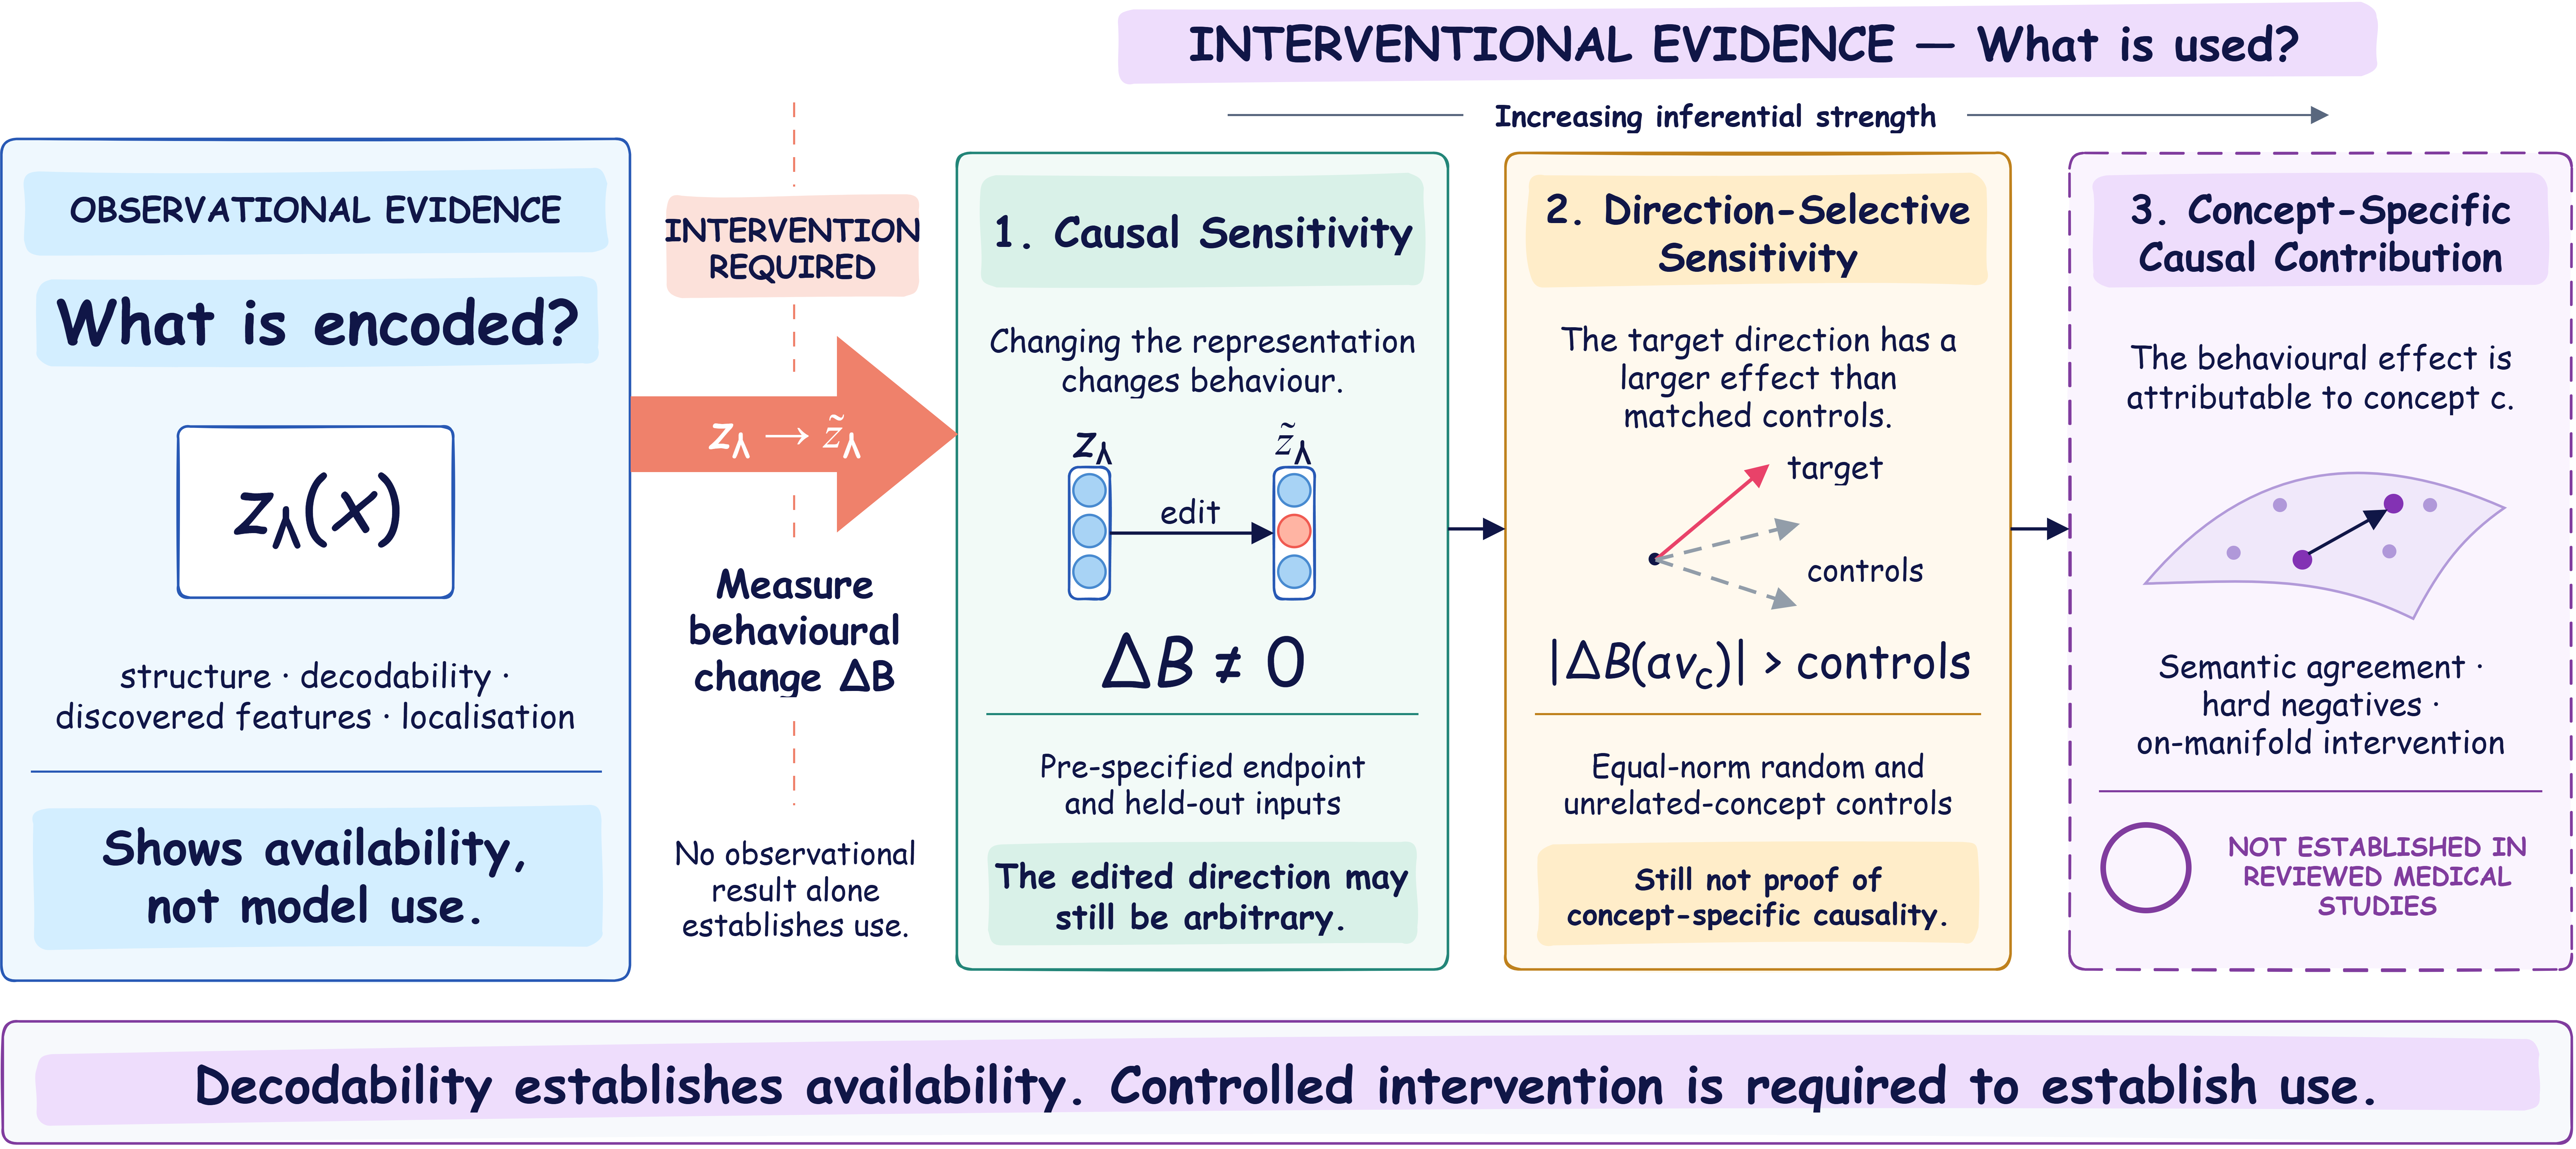
\includegraphics[width=0.95\linewidth]{figures/Figure5_Illustrated.png}
\caption{From what is encoded to what is used. Observational evidence (structure, decodability,
discovered features, localisation) characterises $z_\lambda(x)$ and shows availability, not use. Use
requires an intervention $z_\lambda\to\tilde z_\lambda$ with a pre-specified behavioural end-point
$\Delta B$, and the interventional evidence then climbs the three rungs of
\S\ref{sec:causal-claims}. No reviewed medical study reaches the top rung.}
\label{fig:families}
\end{figure*}

\subsection{Properties evaluated}
\label{sec:eval-what}

The properties below recur across the corpus, and none substitutes for another.

\textbf{Faithfulness and probe validity.} A faithful artefact reflects the computation the model
performs~\cite{jacovi2020towards}. For a probe, a direction or a feature this means connecting the
artefact to the output through an intervention (\S\ref{sec:intervention}); how a removal procedure is
chosen already reorders attribution methods~\cite{hooker2019benchmark}, and fidelity and sensitivity
measures are themselves choices~\cite{yeh2019fidelity}. Probe validity is the weaker property that the
probe's performance reflects the representation rather than the decoder's own work. It is tested by
control-task selectivity, description-length probes or shuffled
labels~\cite{hewitt2019designing,voita2020information}, and a randomly initialised encoder calibrates what
the architecture alone affords. Perturbation and model randomisation test attribution and
attention~\cite{adebayo2018sanity}, tests that medical saliency and attention maps can
fail~\cite{arun2021trustworthiness,sadanandan2026attention}.

\textbf{Concept validity.} Concepts from label schemas, reports or language models may be invalid.
Evaluation covers agreement with expert annotation, inter-rater reliability, whether the concept set is
complete enough to account for the prediction~\cite{yeh2019completeness}, the coverage of the clinical
vocabulary and, for post-hoc names, agreement between descriptions and reports as judged by a frozen
medical language model~\cite{haque2026medconcept}. Plausibility, whether a clinician finds an
explanation reasonable, is a property of the reader and is independent of
faithfulness~\cite{jacovi2020towards,miller2017explanation}.

\textbf{Stability.} Discovered features and learned directions depend on seeds, dictionary size, training
subsets and model versions; reproducibility across seeds, agreement of directions across checkpoints and
consistency of probing across splits measure it (\S\ref{sec:discovery}).

\textbf{Specificity of interventions.} An intervention is evaluated against the three causal claims of
\S\ref{sec:causal-claims} (\S\ref{sec:intervention}).

\textbf{Clinical utility.} The four properties above are functionally grounded; utility is the
application-grounded end of the same scale~\cite{doshivelez2017towards}. An artefact has clinical utility
when it helps a clinician or a developer decide better, measured by reader studies, task-level end-points
such as shortcut detection or error correction, and downstream metrics after an intervention. The
contextual literature includes one dermatology reader study (\S\ref{sec:eval-bench}), and systematic
reviews find mixed, sometimes bidirectional, effects of explanations on trust and
performance~\cite{rosenbacke2024how}.

\textbf{How often the five are reported.} Reporting is uneven, and three gaps stand out. Probe validity is almost never tested: a permuted-label null or chance
calibration appears in \Nprobectrl{} of the \Ndecni{} non-intrinsic decoding studies and a randomly
initialised encoder in \Nproberand{}, and no study runs a control task. Stability is reported by
\Nsaestab{} of the \Nsae{} dictionary studies, and the cross-seed identity of features or names by none;
nor does any decoding, geometry or intervention study establish it for a probe or a direction. And no
core study assesses clinical utility with a reader study. Clinician-facing explanation has been argued to
fail at exactly this step, where an artefact that looks reasonable is taken for one that is
faithful~\cite{ghassemi2021falsehope}. The corpus therefore rests largely on uncontrolled decodability
and on feature names that are unvalidated or validated once (\S\ref{sec:findings}).

% \FloatBarrier  % dropped: it ended the page at the section break and left the right column short
\section{Methods and their medical evidence}
\label{sec:methods}

Each subsection below defines a family, reviews representative studies, tabulates the medical evidence
and states what the family's claims can and cannot support. A study with claims in two families appears
in both. ``Medical'' here means analysing a medical foundation model (\S\ref{sec:models}); general-domain
studies are cited where they supply a method or a mechanism that the medical work uses.
Table~\ref{tab:families} summarises what each family shows and the tests that strengthen it. A core
study whose quality assessment records a defect that undermines its representation-level result
(\S\ref{sec:findings}) is marked $^{\dagger}$ where it is cited singly in this section, so that its
result is read with that qualification.

\subsection{Structural and geometric analysis}
\label{sec:geometry}

Structural analyses characterise a representation space through the arrangement of image and text
embeddings, the spread of the distribution, similarity across models, organisation by scanner or site,
and change under adaptation. They fit no decoder, and they are the cheapest analyses. Only studies that link their statistic to
decodability, retrieval, transfer or shortcut behaviour~\cite{geirhos2020shortcut} are eligible
(\S\ref{sec:method}), so the statements this family supports (F3c, F5, F5b, F6, F11) describe
task-linked geometry alone.

\subsubsection{Modality gap and cross-modal alignment}

\textbf{The modality gap.} Contrastive dual encoders keep image and text embeddings apart, and the gap
is usually measured as the distance between the two modality centroids,
$\Delta=\|\bar z_v-\bar z_t\|_2$, after unit-normalising each embedding. General-domain accounts trace
it to initialisation cones, information imbalance, sparse cross-modal atoms or a functional
role~\cite{liang2022mind,schrodi2025two,dhimoila2026crossmodal,yan2025beyond}. Restrepo \emph{et
al.}~\cite{restrepo2026cone} find tighter cones on medical than on natural data for all four backbones
they test and a smaller cross-modal separation in BiomedCLIP and MedSigLIP than in CLIP and SigLIP,
although the gap persists; shifting the frozen embeddings gives task-dependent gains below 0.02 AUROC,
without a random-direction control. Gap-shrinking losses and gaze guidance improve retrieval, captioning
and alignment~\cite{grassucci2025closing,lahmar2026bridging,kumar2024improving}, each on its own protocol.

\textbf{Alignment quality.} Contrastive objectives decompose into alignment and
uniformity~\cite{wang2020understanding}, and intra- and cross-modal similarities disagree in
CLIP~\cite{mistretta2025cross}. In medical models, global alignment survives where local alignment does
not: in GLoRIA, global image--sentence similarity separates the paired sentence from a random one in
70\% of cases, region-level similarity in only 55\%, and in 43\% on abnormal pairs, below
chance~\cite{mcinerney2022that}. Counterfactual edits of negation and laterality barely move BiomedCLIP
and PubMedCLIP similarity~\cite{balogh2026regularization}$^{\dagger}$, and a projection head can collapse
tumour and normal prototypes to 98\% similarity~\cite{arora2026semantic}. Because distinct patients
share findings, many off-diagonal negatives are semantically positive; the objectives that address
this~\cite{wang2022medclip,park2025off,zhang2025fane,ztrk2025meta} are evaluated downstream rather than
geometrically.

\subsubsection{Anisotropy, effective rank and dimensional collapse}

The cone effect, anisotropy, low effective rank and dimensional collapse all describe concentration of
the embeddings in a small subspace, first found in language embeddings~\cite{ethayarajh2019how}.
Effective rank, $\mathrm{erank}=\exp(-\sum_k p_k\log p_k)$ with $p_k$ the normalised singular values of
the centred embedding matrix, summarises it~\cite{roy2007effective,garrido2022rankme,rudman2022isoscore},
and contrastive training can collapse dimensions~\cite{jing2021understanding,hassanpour2024overcoming}.
The one medical test of whether this structure matters is indirect: across eight encoders, aggressive
post-hoc whitening lowered downstream AUC in 34 of 36 model--dataset pairs, whereas gentler spectral
standardisation gained about 0.005 AUROC~\cite{garciahidalgo2026embedding}. Since the near-isotropic
encoder degraded with the rest, the experiment does not show that the anisotropy itself is the
task-relevant structure, and F5 records the point as a single-study hypothesis. Concentration neither
places concept directions in the dominant subspace nor prevents decoding along low-variance directions,
so similarity scores need standardisation and, under superposition~\cite{elhage2022toy}, overcomplete
dictionaries (\S\ref{sec:discovery}).

\subsubsection{Cross-model similarity}

Cross-model similarity is measured by linear centred kernel alignment
(CKA)~\cite{kornblith2019similarity}, representational similarity analysis
(RSA)~\cite{kriegeskorte2008representational}, canonical-correlation
measures~\cite{raghu2017svcca,morcos2018insights} or Procrustes distances, whose sensitivities differ and
are benchmarked elsewhere~\cite{klabunde2023similarity,ding2021grounding}. Under the
platonic-representation hypothesis~\cite{huh2024platonic}, visual tokens align with text through the
stack~\cite{neo2024towards}, whereas pathology encoders track the slide of origin over
disease~\cite{mishra2025comparing}.

The largest medical study examines 18 image and 7 text encoders across five modalities in an
objective-stratified training matrix~\cite{tayebiarasteh2026self}. Convergence is modest and groups by
objective rather than scale: matched self-supervised encoders align most (40.4\% on chest radiography),
label-supervised ones less (21.1\%) and image--text ones least (3.3\%), and no image encoder aligns with a
clinical text encoder, although linear classifiers transfer at about 85\%. Across 22 encoders and 20
datasets, chance-calibrated nearest-neighbour discordance puts blind sets above a hypergeometric null for
almost every pair of medical datasets, against about half of natural-image
pairs~\cite{arasteh2026candor}, a statistic that hubness distorts in high
dimensions~\cite{radovanovic2010hubs}. Elsewhere, between-scanner reliability of brain encoders is
poor, CKA falls under MRI artefacts while effective rank holds, nearest-neighbour overlap among
volumetric encoders tracks model quality, and an affine map stitches frozen chest-radiograph encoders
into a zero-shot
classifier~\cite{navarrogonzalez2026crossscanner,mielcarz2026do,aerts2025foundation,folco2025semantic}.
None of this is surprising if training pipelines are underspecified: equal downstream performance does
not identify equivalent representations~\cite{damour2022underspecification}, and identifiability up to
a linear map holds only under conditions that these pipelines do not check~\cite{roeder2020linear}.

\subsubsection{Site, scanner and acquisition structure}

Acquisition confounding predates foundation models~\cite{zech2018variable}, and medical embeddings are
organised the same way (\S\ref{sec:decoding}~\cite{dejong2025current,komen2024do,zheng2024demographic}).
The signatures behave as geometric distortions: one affine correction per model harmonises embeddings
across pathology scanners and MRI field strengths~\cite{donle2026featmap}, scanner variability shifts
calibration while preserving discrimination~\cite{thiringer2026scanner}, and a contrastive projection on
frozen embeddings reduces scanner clustering~\cite{carloni2025pathology} (\S\ref{sec:intervention}).

Pathology provenance is recoverable at high accuracy. Source hospital is decodable from ten encoders at
AUC 0.82--0.99, site above 0.95 after stain normalisation, scanner from slide embeddings above 0.99, and
14--55\% of a patch embedding's neighbours reflect the centre rather than the
biology~\cite{zhang2025hospital,murchan2024deep,kmen2026robust,jung2026foundation,shafique2026investigating,saueressig2025histology,gustafsson2024evaluating,esbri2025benchmarking}.
The consequence goes beyond detectability. The scanner signature covaries with case mix and inflates an
external Ki-67 correlation~\cite{jung2026foundation}; stain normalisation, lossy DICOM conversion and
sequential sectioning all move embeddings and
predictions~\cite{wolflein2023benchmarking,mayer2025lossy,balan2025reproducibility}; and in CT and PET,
embedding concordance holds across reconstruction settings while nodule-outcome ranking moves with
them~\cite{park2025evaluating,farquhar2026pretraining}.

Outside pathology, frozen Mammo-CLIP features cluster by dataset across ten mammography cohorts, and
the encoder most organised by cohort probes best yet loses most under external transfer, ending level
with a general encoder~\cite{germani2025bias}. Six further studies tie embedding structure to subgroup
and imaging attributes, judged image quality, tissue-type clustering, augmentation, biological order and
institutional
artefacts~\cite{alloula2025representation,ouaari2026assessing,fournier2026prognostic,elphick2024are,vig2026do,zhang2026auditing},
and image--report correspondence in a chest-radiograph joint space, at 15--50 times chance, is a
re-linkage risk~\cite{tayebiarasteh2026crossmodal} (\S\ref{sec:applications}).

\subsubsection{Representation change under adaptation}

Similarity, checkpoint probes and cross-model dictionaries measure how a representation changes under
fine-tuning, low-rank adaptation and continued pre-training. General-domain work finds that fine-tuning
changes the top layers most and can distort features, that low-rank updates introduce intruder
dimensions, and that visual instruction tuning moves visual features into intermediate language-model
layers~\cite{merchant2020what,zhou2021closer,kumar2022fine,lee2022surgical,raghu2019rapid,biderman2024lora,shuttleworth2024lora,palacios2026visual,verma2024cross}.
Medical few-shot and meta-learning methods are assessed downstream only~\cite{bo2025famnet,wang2025task},
and the three representation-level medical studies measure cross-hospital drift, forgetting during
continued pre-training, and adapter placement from transferred
dictionaries~\cite{theofilou2025stable,zoellin2024block,sadanandan2026mechanistically}. Whether concept
directions survive transfer is unmeasured; crosscoder model diffing~\cite{minder2025overcoming} offers
an instrument (\S\ref{sec:discovery}).

\subsubsection{Summary and discussion}

Medical encoders converge modestly and group by objective rather than
scale~\cite{tayebiarasteh2026self}; in one study an affine map aligned them to within about a dozen
AUROC points of the source encoder~\cite{folco2025semantic}; and they place acquisition variables in
prominent directions. \Vgeoany{} of the \Vgeon{} geometry records compare their statistic with a
comparison model or a null. Whether geometry-modifying methods repair what they target is unmeasured,
because they are assessed only downstream.

\subsection{Supervised concept mapping and decodability}
\label{sec:decoding}

Decoding maps a representation to an external concept through a probe, a concept activation vector,
similarity to a labelled set or zero-shot text scoring. It is the oldest family, and what it measures is
decodability, a joint property of the representation and the
decoder~\cite{alain2016understanding,belinkov2021probing,hewitt2019designing,elazar2020amnesic}.

\subsubsection{Probing for clinical findings and anatomy}

Seventeen frozen-feature benchmarks meet the criteria of \S\ref{sec:method}, \Nbenchdec{} of them with
decoding records and two with structural records only. They rank frozen pathology, chest-radiograph, CT,
retinal and volumetric
encoders~\cite{neidlinger2025benchmark,marza2025thunder,li2025featurequality,li2025embeddings,chevli2026frozenct,zhou2025generalist,aerts2025foundation}.

What such probes can and cannot tell is visible in three studies. Across ten mammography cohorts, frozen
Mammo-CLIP probes beat GLoRIA, CLIP and DINOv2 by 9.7 to 15.3\% relative F1, yet a probe fitted on a
single cohort falls from 0.73 to 0.32 on the other nine~\cite{germani2025bias}. On 492,724 chest
radiographs, pooled embeddings from five frozen transformers are at chance for controlled small-scale
perturbations while patch tokens from the same forward pass recover them; but the patches are selected by
the ground-truth lesion box, so the recovery is an oracle readout rather than a deployable
one~\cite{muthyala2026frozen}. On a pre-registered PET benchmark of 2,592 patients, patch classification
saturates for every frozen encoder and for a randomly initialised control~\cite{farquhar2026pretraining}.

The same readout reaches phenotype codes, training configurations, tissue and cell types, omics tasks,
placental lesions, prostate grade, kidney morphometrics and radiological retrieval, in benchmarks of
five to nineteen
encoders~\cite{lin2026transparent,liang2026cheap,demir2025downstream,cui2026translating,hu2026probing,jamzad2026p3ca,sadman2025interpreting,svatko2026deep,jung2026foundation,steiner2026when,vadori2025mind,bakhta2026frozen,beyeler2024comparing,peng2025benchmarking,gustafsson2024evaluating,kasireddy2025explainable,denner2024leveraging,howard2024generative,ramchandani2026benchmarking,zhao2026benchmarking}.
The most instructive case is a failure: an ejection-fraction probe with $R^2$ 0.63 in the development
cohort correlates negatively with the label on an external one~\cite{akanova2026interpreting}$^{\dagger}$.
Decodability can also be localised, to intermediate layers for chest-radiograph shortcuts, to a
dictionary neuron for tumours, and to roughly ten channels whose ablation removes a finding
altogether~\cite{pedersen2026look,tamura2025patch,nooralahzadeh2026sparse,goetze2025prediction,basu2026interpretability,nooralahzadeh2026arbitration}.

\subsubsection{Probing for demographic and acquisition attributes}

Before foundation models, medical classifiers were already known to underdiagnose underserved groups,
to rely on hidden strata and acquisition cues, and to predict race, sex and age without anatomical
correlates~\cite{seyyedkalantari2021underdiagnosis,oakdenrayner2019hidden,degrave2020ai,banerjee2021ai,adleberg2022predicting,korot2021predicting,coyner2021color,burns2023ability,vaidya2024demographic,jones2024causal}.
Asking whether an attribute is encoded or used made this a representation-level
question~\cite{glocker2023algorithmic,glocker2022risk}.

Frozen CT embeddings trained without demographic labels decode sex at AUROC 0.998, age at RMSE 3.8 years
and race at 0.878~\cite{zheng2024demographic}. The pattern recurs in chest radiography, pathology, brain
MRI, retina and mammography, where embeddings also give away site, camera or dataset, even after stain
normalisation~\cite{sourget2025fairness,dejong2025current,komen2024do,rahbar2026frozen,li2026acquisition,hajishafiezahramini2026dataset,encin2026comparative,lin2025beyond,kmen2026robust}.
The range is wide. Eight chest-CT encoders decode race at only 0.72--0.74 AUROC and read age and sex no
better than a randomly initialised encoder~\cite{tariq2024self}$^{\dagger}$, and of thirteen shortcut
detectors on CheXpert only the non-probe ones flag race~\cite{cajas2026shortkit}.

Availability and use come apart here too. On 230,697 radiographs, sex is encoded at AUROC 0.942, yet
linear finding probes refitted after residualising it out lose less than 0.001 AUROC; the sex component
is redundant for an optimally refitted linear readout, and whether the model's own head used it was not
tested~\cite{kim2026encoding}$^{\dagger}$. Orthogonalisation recovers these attributes before projection
and chance after, cropping reduces them, and fairness benchmarks span 17 datasets and 20
models~\cite{weber2023posthoc,sutariya2026impact,jin2024fairmedfm,kauffmann2024explainable}.

\subsubsection{Concept activation vectors and directional sensitivity}

Concept activation vectors (CAVs) fit a direction $v_c$ from labelled positive and negative examples and
score a class by the directional derivative of its logit along $v_c$; the TCAV score is the fraction of
inputs with a positive derivative, tested against random directions~\cite{kim2018interpretability}.
Applications cover histopathology, dermoscopy, cardiac MRI and diabetic-retinopathy
grading~\cite{graziani2018regression,graziani2020concept,lucieri2020interpretability,clough2019global,stors2024looking},
and iterated HPV directions predict HPV status in a pathology
encoder~\cite{hieromnimon2025analysis}$^{\dagger}$. Text-derived vectors remove the need for labelled
exemplars and support adversarial debiasing~\cite{nicolson2024textcavs,correa2023efficient}, but the
scores stay observational, and they are inconsistent across layers, entangled and spatially
dependent~\cite{nicolson2024explaining}.

\subsubsection{Representational similarity with concept-labelled sets}

Representational similarity analysis compares distances in the representation with distances between
stimuli, without a decoder~\cite{kriegeskorte2008representational}. Across six pathology encoders,
similarity follows slide identity more than disease~\cite{mishra2025comparing}; diffusion pseudotime over
five pathology encoders recovers the progression order of four cancer types against a label-shuffled
null~\cite{vig2026do}; and chance-calibrated discordance across 22 encoders shows one encoder reading
pneumothorax at 84.5 AUROC while placing 18\% of positives nearer an opposite-label film from the same
hospital~\cite{arasteh2026candor}.

\subsubsection{Text-anchored concept scoring}

Prompt similarity in a joint space gives zero-shot concept scores. MONET audits data and models with
dermatologist-verified concepts~\cite{kim2024transparent}, and pre-training on 23 million
image--text--concept triplets extends the approach~\cite{nie2025explainable}. The same scoring serves as
a general-purpose concept detector, for dermoscopic criteria, retinal clusters, concept-to-region
grounding and counterfactual
generation~\cite{patricio2023conceptbased,mensah2026interpretable,luo2025xbench,sadashivaiah2024explaining},
with one instructive limit: it detects injected biases but not implicit
ones~\cite{bertolini2025strengths}. Because the prompt alters the direction, expert-label validation is
required (\S\ref{sec:eval-what}).

\subsubsection{Validity controls}

An expressive decoder needs a control: a control task refits $\mathcal G$ in~(\ref{eq:probe}) on
permuted or type-matched labels and reports the difference~\cite{hewitt2019designing}, description
length controls capacity~\cite{voita2020information}, and amnesic probing and erasure test whether
removing a property changes
behaviour~\cite{elazar2020amnesic,ravfogel2020null,belrose2023leace,pimentel2020informationtheoretic,guerner2023geometric}.
Medical use of these controls is rare. Among the \Ndecni{} core decoding studies outside intrinsic
designs, \Nprobectrl{} report a shuffled-label null or a chance
calibration~\cite{liang2026cheap,rahbar2026frozen,vig2026do,bertolini2025strengths,arasteh2026candor,steiner2026when,li2026acquisition,cajas2026shortkit},
none a control task in the sense of Hewitt and Liang, and \Nproberand{} report a randomly initialised
encoder~\cite{rahbar2026frozen,arasteh2026candor,svatko2026deep,farquhar2026pretraining} and
\cite{tariq2024self}$^{\dagger}$. Twenty-eight compare medical and general models on the same data.
Only four probe successive depths to localise where a concept becomes
decodable~\cite{pedersen2026look,rahbar2026frozen,vig2026do,vadori2025mind}, two more read several
depths without localising~\cite{farquhar2026pretraining,demir2025downstream}, one varies pooling rather
than layer~\cite{muthyala2026frozen}, and the rest probe the final embedding; a frozen-probe benchmark
of physiological-signal models shows what a complete protocol looks like~\cite{zare2026eeg}.

\subsubsection{Summary and discussion}

Clinical findings, anatomy, demographic attributes and acquisition conditions are all decodable from
frozen medical encoders. Whether a recoverable attribute influences the output is usually untested: only
residualisation~\cite{kim2026encoding}$^{\dagger}$ and channel ablation~\cite{nooralahzadeh2026sparse}
separate availability from the dependence of a specified downstream readout, and neither tests the
model's own fixed head. Decodability of a named concept across successive loci of one model, under a
control, remains unmeasured; the one successive-locus probe reads class labels without one (F8b,
\S\ref{sec:tracing}).

\subsection{Feature decomposition and discovery}
\label{sec:discovery}

Discovery decomposes a representation into neurons, factorised directions or sparse features without a
prior vocabulary, and then names them from the inputs that activate them. What the family establishes
depends on whether the names are valid and the features stable.

\subsubsection{Neuron-level analysis and network dissection}

Network dissection labels each unit with the concept whose mask best overlaps its activation
map~\cite{bau2017network}; CLIP-Dissect substitutes a vision--language model for the labelled
masks~\cite{oikarinen2022clipdissect}, and the multimodal neurons of CLIP are the precursor of
unit-level multimodal discovery~\cite{goh2021multimodal}. Mid-layer atlases of a pathology encoder show
coherent tissue concepts but dispersed subclasses, with pathologist agreement falling from $\kappa$ 0.82
for cancer groups to 0.11 for subclasses~\cite{gustav2026class}; other unit-level work labels
mammography neurons, rebuilds a diagnostic model, probes retinal networks and reads hallucination off
language-model
units~\cite{salahuddin2025mammoclip,gong2025concepts,yousefzadeh2023lava,vankadaru2026readable}. The
limits of unit analysis are well known: superposition and non-axis-aligned
concepts~\cite{elhage2022toy,park2023linear}, concepts carried by combinations of filters rather than by
one~\cite{fong2018net2vec}, and the non-identifiability of unsupervised factors without inductive bias or
supervision~\cite{locatello2019challenging}. Medical work has therefore moved to dictionaries.

\subsubsection{Factorisation directions}

Principal components, independent components and non-negative factors give a few directions, and in
medical embeddings these reflect acquisition and site before pathology (\S\ref{sec:geometry}): among
inverted principal components of pathology-encoder gradients, one stain-colour direction carries
54--69\% of the tissue-source-site gradient, against at most 20\% for any grade
component~\cite{howard2024generative}. Other factorisations recover plausible morphology: concept-bank segmentation beats a
ResNet-50~\cite{gildenblat2024segmentation}$^{\dagger}$, three pathologist-named HPV-positive subtypes
emerge~\cite{hieromnimon2025analysis}$^{\dagger}$, and carcinoma morphology, retinal characteristics,
breast-cancer archetypes and an infectious-disease proposal are reported
alongside~\cite{qin2026clearhpv,varshney2024generating,beyeler2024comparing,fournier2026prognostic,sizikova2022automatic}.
Activation clustering~\cite{ghorbani2019automating,fel2023a} and sparse decomposition onto a fixed
vocabulary~\cite{bhalla2024interpreting} have no medical instance.

\subsubsection{Sparse autoencoders and dictionary learning}

A sparse autoencoder (SAE) reconstructs activations through an overcomplete, sparsely active layer of
candidate monosemantic features~\cite{cunningham2023sparse}. With codes
$a(x)=\sigma(W_e z_\lambda(x)+b_e)$ and reconstruction $\hat z=W_d\,a(x)+b_d$, the dictionary
minimises
\begin{equation}
\begin{split}
&\mathbb{E}_x\big[\|z_\lambda(x)-\hat z(x)\|_2^{2}+\beta\,\|a(x)\|_1\big]\\
&\quad\text{s.t.}\ \|(W_d)_{:,j}\|_2=1\ \forall j,
\end{split}
\label{eq:sae}
\end{equation}
where $(W_d)_{:,j}$, the $j$th column of the decoder, is the direction of feature $j$. The reviewed
medical dictionaries replace the $\ell_1$ penalty by a fixed active-code count, a gated or jump
activation or a crosscoder loss; this changes what is held fixed, not the estimand. Each column is
named from its highest-code inputs, a route that need not identify what the feature does, since the
maximally activating patches of a feature can fail a causal test of the same
feature~\cite{han2025causal}. Dictionary learning grew out of the monosemanticity
work~\cite{bricken2023monosemanticity,templeton2026scaling}, and scaling~\cite{gao2024scaling}, better
activations~\cite{rajamanoharan2024jumping} and open dictionaries~\cite{lieberum2024gemma} made SAEs
portable. Dictionaries that decompose an image--text space
jointly~\cite{kaushik2026decomposing,gordon2026scocca} address the cross-modal case that the modality
gap of \S\ref{sec:geometry} makes hard; no reviewed medical study uses one.

Medical adoption has come in two waves. The first trains on \emph{frozen encoders}. Pathologists curated
41 sarcoma concepts on CONCH embeddings, where the full dictionary reaches 73.7\% balanced accuracy
against 77.4\% for the raw aggregator and 67.0\% for the curated
concepts~\cite{bisson2026unsupervised}$^{\dagger}$. Others take names from report-distilled
descriptions, tissue structures, pathologists, radiologist regions or an automated
labeller~\cite{abdulaal2024an,le2024learning,kim2026dissecting,zhao2026compositional,redlich2026explainable,nakka2025mammosae,renzulli2025medsae,tang2025cxrlanic,sun2025prototypebased,dasdelen2025cytosae,yan2026a,huang2026classguided,chhetri2026when},
and the dictionaries compress: ten features recover most downstream CT and MRI
performance~\cite{wesp2026sparse}, and a geometry-guided dictionary predicts Alzheimer's
conversion~\cite{nerrise2026geosae}.
The second wave trains on the \emph{residual streams of medical multimodal LLMs}: device, pathology and
longitudinal-change features from a report generator~\cite{bouzid2025insights}, steering directions on
three radiology models~\cite{nooralahzadeh2026universal} (\S\ref{sec:intervention}) and a transferable
general suite~\cite{sadanandan2026mechanistically}; domain-specific dictionaries explain more of the
clinical activation variance~\cite{oneill2025resurrecting}. No eligible medical study trains a dictionary
across models, across modalities or on model differences, although the templates exist in general
work~\cite{thasarathan2025universal,nasirisarvi2025sparc,minder2025overcoming,plantinga2025from}, in
dictionaries over medically fine-tuned language, segmentation and physiological-signal
models~\cite{tan2026efficient,ahmed2026medseglens,lehnschiler2026mechanistic,duan2026cadence}, and in
general-vision dictionaries that steer or segment through the visual
stream~\cite{joseph2025steering,pach2025sparse,stevens2025interpretable} (\S\ref{sec:future}).

Across the \Nsae{} core dictionary studies, every axis that fixes a feature varies: token, layer,
expansion and sparsity. Features are therefore not commensurable across studies, and naming is as
uneven. Feature meaning is validated by clinician readers in \Nsaeclin{} studies and by structured labels
in \Nsaelabel{}, and only the \Nsaeval{} with either kind of validation enter statement F7
(\S\ref{sec:findings}). Only \Nsaestab{} report a reproducibility check, none matches features across
seeds, and only \Nsaerecon{} quantify reconstruction. The headline claims of ten-feature
compressibility~\cite{wesp2026sparse} and five thousand monosemantic features~\cite{tang2025cxrlanic}
are thus neither validated nor reproduced.

\subsubsection{Naming, validation and stability}

Automated pipelines name features from activating inputs and score the
names~\cite{paulo2024automatically}. The medical instances grade names against reports, labels or
regions, or discover features first and name them
afterwards~\cite{bouzid2025insights,abdulaal2024an,haque2026medconcept,nakka2025mammosae,rao2024discover};
none tests agreement between labellers. Stability is the larger problem. Absorption and splitting persist
across widths and sparsities~\cite{chanin2024a}, differently seeded dictionaries share about 30\% of
their features~\cite{paulo2025sparse}, derived concepts are adversarially fragile~\cite{li2025evaluating},
and the metrics and benchmarks are too unstable to separate
architectures~\cite{chanin2026are,chanin2026synthsaebench}. In an event-sequence anchor few features
reproduce and dictionary probes do not beat dense ones~\cite{sainsbury2026sparse}, and capacity-matched
suites are proposed for signal models~\cite{duan2026ecginterpbench}. A named feature is a hypothesis, not
a stable identifier, although reconstruction of the subspace survives.

Dictionaries trained on encoder activations recover much of what probing already sees, and do so
without a concept vocabulary fixed in advance. No study yet decomposes the connector output, and none
matches features across cohorts.

\subsection{Representation attribution, localisation and tracing}
\label{sec:tracing}

Tracing observes the forward pass without changing it. It localises a concept to a layer, a position, a
head or a training example, and each localisation is a hypothesis for later patching or steering. The
medical studies mostly ask where multimodal LLMs use the image.

\subsubsection{Residual-stream decomposition and lenses}

The logit lens reads an intermediate state through the unembedding matrix; the tuned lens learns a
layer-specific affine map first~\cite{belrose2023eliciting}. In vision--language models, visual tokens
become text-decodable and the middle layers enrich and then refine them, while visual information
declines across layers and generation steps~\cite{neo2024towards,jiang2024devils,li2025the}; objects are
named without fine-grained comparison, and steering vectors leave no lens-decodable
trace~\cite{shahgir2026vlms,nadaf2026steerable}. Medical lenses track the formation of a diagnosis in a
breast-cancer transformer~\cite{takahashi2026vision}, place multilingual knowledge at intermediate
layers but not at the output~\cite{abouzahir2026bridging}, and find visual attributes early regardless of
whether the answer is correct~\cite{nooralahzadeh2026arbitration}.

\subsubsection{Attention, visual tokens and the connector}

Attention to the image is measured as the attention mass on visual tokens, summed over heads and
layers, or by rollout and its refinements~\cite{abnar2020quantifying,chefer2021transformer}. None of these
quantifies a causal contribution, as the attention-as-explanation debate
established~\cite{jain2019attention,wiegreffe2019attention,serrano2019is}. General-domain work finds
middle-layer concentration on real objects, staged flow into the question tokens, attention sinks,
redundant visual tokens and modality-specific
neurons~\cite{jiang2024devils,zhang2024cross,kang2025you,luo2025sink,chen2024image,wang2025token,huo2024mmneuron,huang2024miner,kang2025large,kim2025interpreting,jiang2025investigating}.
Connectors map correlated embeddings into the language model's feature
space~\cite{lee2026more,venhoff2025visual} and hallucinate when they are over-aligned to
text~\cite{fan2026visual,venhoff2025too,saini2026when}; dermatology fine-tuning improves the projection
but not its domain specificity~\cite{verma2024cross}.

Eleven core records from eleven studies, nine of which take tracing as their primary family
(\S\ref{sec:method}), read attention or attribution maps of medical models, and \Vtrany{} test the maps
against perturbation, occlusion or counterfactual evidence. Where they are tested, the maps often fail,
and the result depends on the benchmark and the end-point. Four attribution methods disagree under
patch deletion and insertion across 17 RETFound models, with gradient-weighted rollout best in 11 of
17~\cite{bors2026benchmarking}, and the internal attributions of six vision--language models miss the
counterfactually verified evidence region on chest radiographs, with a rollout IoU of 2.7\% against 39.2\%
for the best gradient method~\cite{xiong2026rethinking}. Attention maps sometimes anti-correlate with
occlusion importance~\cite{sadanandan2026attention}, lose to perturbation and relevance-propagation
explanations~\cite{idaji2026beyond}, enrich for pathway rather than gene
signatures~\cite{srikanthan2026do}, mark pixels outside the body~\cite{hashmi2024towards}, and are
diffuse and insensitive to the prompt~\cite{injarabian2025interpreting}; an EchoPrime probe beats random
masking only by a method-dependent margin~\cite{akanova2026interpreting}$^{\dagger}$.

The remaining records localise without testing. Visual-attention ratios find a visually dominant window
in two medical multimodal LLMs~\cite{chen2026vihd} (\S\ref{sec:intervention}), and class-label probes at
successive loci of fourteen models name four failure modes, among them loss of fidelity at the
connector~\cite{zhu2026lost}. The earliest record audits GLoRIA's text--image attention on Chest
ImaGenome pairs: the map localises above chance (AUROC 69.1) yet barely moves when ``left'' becomes
``right'', and falls only when the reference boxes move, so it is fixed by the
image~\cite{mcinerney2022that}. Text-tower anchors trace negation failure in a chest-radiograph assistant
and in radiology captions~\cite{vu2025improving,abbasi2026layerspecific}. Input audits agree that image
use is weak: a text-only baseline nearly matches the best multimodal model~\cite{lotfinia2026vision},
VQA grounding stays poor~\cite{chen2026grounding}, and grounding failures can be told
apart~\cite{liu2026medical}. No other study measures a medical connector (Fig.~\ref{fig:corpus}b), so
these token-level results transfer only where the projector preserves patch correspondence
(Table~\ref{tab:models}).

\subsubsection{Encoder tokens, aggregators and training-data attribution}

The encoders of Table~\ref{tab:models} carry three further hazards, none of them a core claim. The
high-norm artefact tokens of vision transformers~\cite{darcet2023vision} are unmeasured in DINOv2-recipe
models such as RAD-DINO, UNI and Prov-GigaPath, where they would dominate the patch norms and attention
that probes read. Self-supervised pathology encoders develop heads that attend to morphological
phenotypes~\cite{chen2022self,chen2024generalpurpose,xu2024wholeslide}, qualitative evidence that
morphology was learned. Tile weights of attention-based multiple-instance learning (MIL)
aggregators~\cite{ilse2018attention,lu2020data} are the usual explanation in computational pathology,
partly answered by prototype- and concept-based aggregators
(\S\ref{sec:intrinsic})~\cite{song2024morphological,huy2025interactive}; like decoder attention, none
of the three is confirmed by patching. Attribution to examples is rarer still. Frozen embeddings support
content-based retrieval over 1.6 million radiological images~\cite{denner2024leveraging}, text-based
decomposition attributes CLIP representations to layers, heads and
patches~\cite{gandelsman2023interpreting,balasubramanian2024decomposing} with no medical instance, and
influence functions~\cite{koh2017influence} identify mislabelled data~\cite{hao2020inaccurate},
re-weight noisy labels~\cite{braun2022influence} and have reached a biomedical language
model~\cite{cao2026scalable}. In medical vision their use is limited to curation and leakage auditing
(\S\ref{sec:applications}), where image--report correspondence creates a re-linkage
risk~\cite{tayebiarasteh2026crossmodal}.

Where the tests exist they return the maps unreliable or method-dependent and the image contribution
weak, and in language models the layer that causal tracing singles out is not the layer at which
editing works best~\cite{hase2023does}.

\subsection{Causal intervention and representation control}
\label{sec:intervention}

This family holds three subtypes that share a name but not an estimand, and their records should not be
read as one total. Interventions inside the forward pass change an activation in a fixed model; post-hoc
transformations change what a refitted readout can do with a stored vector; parameter editing and
unlearning change the model's weights and identify no representation-level mediator unless the study
measures one. Each takes a different control (Table~\ref{tab:families}), and each is read against the
three rungs of \S\ref{sec:causal-claims}; no reviewed medical study reaches the third. The methods come from language
models~\cite{vig2020causal,geiger2021causal,geiger2023causal,meng2022locating,meng2022mass,zhang2023towards,turner2023steering,rimsky2023steering,zou2023representation,li2023inference,arditi2024refusal},
and medical claims date from 2025--2026 and remain sparse and decoder-centred
(Fig.~\ref{fig:corpus}b), after an early orthogonalisation of chest-radiograph
embeddings~\cite{weber2023posthoc} and a joint-space edit~\cite{sadashivaiah2024explaining}.

\subsubsection{Ablation and knockout}

Ablation removes a component. Masking the highest-attention 10\% of visual tokens in the visually
dominant decoder layers of two medical multimodal LLMs detects hallucinations (AUC 71.6--78.9 against
68.9--73.0 for the best baseline), while random masking changes little~\cite{chen2026vihd}. Ablating
object-specific visual tokens reduces object identification in general models~\cite{neo2024towards}, and
knockout in frozen CT encoders shows about ten channels carrying each radiological
finding~\cite{nooralahzadeh2026sparse}. Fine-tuning visually critical heads from weak segmentation
labels is a training method and therefore contextual~\cite{chang2025focus}.

\subsubsection{Activation patching and causal tracing}

Causal tracing corrupts a run, restores the clean-run hidden state at one locus and measures how much
of the output recovers; the indirect effect of locus $\lambda$ in~(\ref{eq:effect}) is
$B(x_{\mathrm{corr}};z_\lambda\!\leftarrow\!z_\lambda(x_{\mathrm{clean}}))-B(x_{\mathrm{corr}})$.
Adaptations to vision--language models localise image-conditioned generation to layers and
tokens~\cite{palit2023towards,basu2024understanding,zhang2024cross,li2025causal}. One medical instance
is core, and it patches a feature rather than tracing a corruption: in MedGemma, patching a single
dictionary feature recovers more of the decision margin than random control
features~\cite{sadanandan2026mechanistically} (F9a). No medical clean--corrupted tracing is core; the
closest scales CLIP text-tower updates by causal contribution~\cite{abbasi2026layerspecific}, and
text-only anchors place editing adapters, localise gender and show knowledge failing to reach the
output~\cite{xu2024editing,ahsan2025elucidating,abouzahir2026bridging}. Automated circuit discovery
remains general-domain~\cite{conmy2023automated,syed2023attribution,marks2024sparse,ameisen2025circuit}.

\subsubsection{Steering vectors and representation engineering}

Steering sets $\tilde z_\lambda=z_\lambda+\alpha v$ and measures $\Delta B(\alpha)$
in~(\ref{eq:effect}). The direction $v$ may be a contrastive mean difference, a probe normal or a
dictionary decoder vector, and the controls are an equal-norm random direction or an unrelated concept.
General vision encoders support patch-level steering~\cite{joseph2025steering,stevens2025interpretable},
and CLIP interventions propagate through the projector~\cite{pach2025sparse}.

The medical evidence is mixed. Per-token steering improves a report-quality composite in three radiology
multimodal LLMs, one of which transfers zero-shot to a second corpus~\cite{nooralahzadeh2026universal},
while Matryoshka dictionary steering gives mixed results~\cite{bouzid2025insights}. Contrastive
activation addition, with random and reversed controls, shifts pneumonia classification in one of three
frozen chest-radiograph models~\cite{farina2026translating}; moderate modality-gap shifts improve
supervised performance~\cite{restrepo2026cone}; and lesion-mask amplification improves subtle-lesion
detection across five backbones, although on CT it rests on one model without a random
control~\cite{zeng2026easylens}. Text-only anchors divide in the same
way~\cite{basu2026interpretability,vankadaru2026readable,ahsan2025can,ray2026do}. General-domain work
explains the inconsistency: steering effects are input-dependent, sometimes reverse sign and are not
identifiable~\cite{tan2024steeringreliability,braun2025understanding,venkatesh2026nonident}; random
directions alone raise harmful compliance from 0\% to 1--13\%~\cite{korznikov2025the,li2026analysing};
and function-vector steering dissociates from lens decodability~\cite{nadaf2026steerable}.

\subsubsection{Post-hoc transformation, editing and unlearning}

Editing changes weights, unlearning removes the influence of data, erasure removes concepts, and
post-hoc transformations (whitening, harmonisation, projection, transport) change stored embeddings
before re-evaluation. An operation on a frozen representation with a downstream end-point is core
(Table~\ref{tab:boundary}); a method that changes the encoder's training or weights alone is contextual.
Editing fails on medical benchmarks: gradient-based editors generalise but violate locality,
memory-based editors preserve locality without generalising~\cite{zhu2026evaluating}, and every editor
tested fails under single and sequential editing~\cite{xu2025medmkeb,wen2025multimededit}. Unlearning
is contextual~\cite{guo2026exploring,hardan2025forgetmi,xu2025from}, at best projecting the target
subspace out of language-model and connector weights~\cite{wu2025hierarchy}; mechanistically guided
low-rank adaptation improves paraphrase consistency~\cite{sadanandan2026mechanistically}, and editing
1\% of the weights injects persistent misinformation into a text-only anchor~\cite{han2024medical}.

Null-space projection~\cite{ravfogel2020null,ravfogel2022linear}, linear erasure~\cite{belrose2023leace}
and amnesic probing~\cite{elazar2020amnesic} remove linearly decodable attributes. Projecting
chest-radiograph embeddings off the protected-attribute column space removes attribute effects on
pathology logits and shrinks subgroup AUC gaps, with a macro-AUC change of $-1.4$ to $+1.8$ points across
two model--dataset pairs~\cite{weber2023posthoc}. On retinal embeddings the same operation lowers
device decodability only from 0.95 to 0.70--0.86 and leaves a three-year device shift in predicted
age~\cite{li2026acquisition}. Residualising demographics leaves clinical-finding prediction unchanged,
a test of dependence~\cite{kim2026encoding}$^{\dagger}$; the joint-space analogue edits along
report-derived directions~\cite{sadashivaiah2024explaining}.

In pathology the target is acquisition. Site prediction falls to chance under
ComBat~\cite{murchan2024deep}$^{\dagger}$ and a gradient-reversal head~\cite{zhang2025hospital}$^{\dagger}$,
with biomarker end-points holding; centre-signature removal raises robustness but not
generalisation~\cite{kmen2026robust}; contrastive projection raises same-specimen
agreement~\cite{carloni2025pathology}; an affine correction raises cross-scanner
retrieval~\cite{donle2026featmap}; and whitening degrades downstream
performance~\cite{garciahidalgo2026embedding} (\S\ref{sec:geometry}). Two core joint-space operations do
the same, scoring CPath-CLIP embeddings against text anchors to raise cross-species tumour
transfer~\cite{arora2026semantic} and regularising a text projection head against counterfactual
text~\cite{balogh2026regularization}$^{\dagger}$. Evaluated only downstream, these operations establish
what they remove, not what the model uses (F3b). Adversarial perturbation of frozen embeddings is a
training method~\cite{xu2024apple}, and demographic attributes (\S\ref{sec:decoding}) remain the usual
target of erasure.

Concept-directed effects are specific to the input and the model. No study in this corpus intervenes
on the connector, and because steering effects are not
identifiable~\cite{korznikov2025the,venkatesh2026nonident}, an uncontrolled improvement cannot be
credited to a concept.

\subsection{Intrinsic and concept-aligned designs built on foundation models}
\label{sec:intrinsic}

Intrinsic designs constrain part of a representation to be interpretable by construction. This is a
property of the model, and the analysis of such a model stays in the preceding families: eligible
designs carry the intrinsic-design tag and are coded in the supporting family, decoding in every case
but one discovery-coded prototype design.

\subsubsection{Concept bottlenecks on frozen medical encoders}

A concept bottleneck model (CBM) predicts
human-defined concepts and then the label from the concepts alone, $\hat c=g_c(z_\lambda(x))$ and
$\hat y=g_y(\hat c)$, so that the label depends on the representation only through the inspectable
$\hat c$~\cite{koh2020concept}; concept embedding models relax the bottleneck to a vector per concept to
recover accuracy~\cite{zarlenga2022concept}. Post-hoc and label-free variants attach to pre-trained
encoders, with a language model proposing concepts and a vision--language model scoring
them~\cite{yuksekgonul2022post,oikarinen2023label,yang2022language}. GPT-4 concepts scored by a
vision--language model give classifiers across eight medical datasets~\cite{yan2023robust}, textbook-
and PubMed-derived concept spaces degrade less than black-box fine-tuning on confound-reversed
splits~\cite{yang2024textbook}, and stronger associations in intermediate than in final layers motivate
multi-layer bottlenecks~\cite{wang2025mvp}. Applications reach volumetric, slide and ultrasound
encoders~\cite{rojas2026echopcbm,tushar2026distilling,gao2025evaluating,sun2025label}: frozen-CT ridge
concept heads recover lung-nodule attributes only weakly ($R^2\le 0.24$) yet generalise externally
better than embedding probes. Distribution shift degrades frozen-feature bottlenecks, and concept-layer
adaptation recovers part of the loss~\cite{choi2024adaptive}; VLM-supervised concepts can differ from
expert annotations, and concept accuracy relates only weakly to explanation
quality~\cite{debole2025if} (\S\ref{sec:eval-what}).

\subsubsection{Concept-based vision--language models and report-grounded bottlenecks}

Here the concept layer
sits inside a medical VLM. Radiologist-style observation probabilities yield zero-shot
diagnoses~\cite{pellegrini2023xplainer}, elicited criteria become textual anchors in the joint
space~\cite{gao2024aligning} or explainable prompts~\cite{bie2024xcoop}, and large VLMs classify from
their own answers to concept questions~\cite{patricio2025cbvlm}. A two-step variant reads dermoscopic
concepts off frozen MONET image--text similarity and passes them to a language model, beating a trained
bottleneck on three datasets; ground-truth concepts add 5--21 points, and BiomedCLIP concepts are at
chance~\cite{patricio2025twostep}. Report-derived concepts in a chest-radiograph joint embedding provide
counterfactuals~\cite{sadashivaiah2024explaining}, guideline text supports conformant classification in
a general CLIP model~\cite{harmanani2026vision}, and a radiology foundation model projects chest
radiographs into a language-model concept space validated on physician-annotated
cohorts~\cite{han2026clear}.

\subsubsection{Prototype and part-based models on foundation features}

Case- and part-prototype models explain
by similarity to exemplars~\cite{chen2019thislooks,barnett2021case,kim2021xprotonet}. Foundation-model
versions summarise slide patch embeddings into morphological prototypes~\cite{song2024morphological} or
give patch-level prototypes an interactive concept meaning~\cite{huy2025interactive}; a
self-interpretable multiple-instance model pairs handcrafted and deep branches~\cite{kapse2023si};
region-additive logistic heads on frozen BrainIAC and NeuroFM embeddings of anatomically masked
volumes match fine-tuning while randomised embeddings fall to chance~\cite{zhang2026regionfm}; and
attribute-regularised or concept-whitened spaces align axes with clinical
attributes~\cite{cetin2022attri,hou2024concept}, the medical instances of concept
whitening~\cite{chen2020concept}. Because prototypes and aligned axes are points and directions in
feature space, they are evaluated by decoding and discovery.

\subsubsection{Critiques}

Intervening on a bottleneck requires the label to depend only on the concepts, yet
the concept predictors may ignore the relevant regions~\cite{margeloiu2021do} and soft scores leak
non-concept information~\cite{havasi2022addressing}. Random concept projections match the accuracy of
learned ones, so accuracy cannot certify meaning~\cite{srivastava2024vlg,schmalwasser2026faithfulness};
information-theoretic measures quantify the leakage~\cite{parisini2025leakage,makonnen2025measuring},
and intervenability extends beyond bottlenecks~\cite{marcinkevics2024beyond}. Inconsistent dermoscopy
annotations cap hard-bottleneck accuracy~\cite{napoles2026concept}, and concept accuracy can conceal a
meaningless layer~\cite{han2026loss}. A sparse autoencoder placed before a linear
bottleneck~\cite{rao2024discover} inherits the instability of discovery (\S\ref{sec:discovery}).

Where the comparison is reported, task accuracy is competitive with the same backbone without the
concept layer, but accuracy cannot show faithfulness. The two controls the corpus does contain are an
embedding-randomisation null~\cite{zhang2026regionfm} and the replacement of predicted concepts by
ground truth~\cite{patricio2025twostep}.

\subsection{Comparison across families}
\label{sec:comparison}

\begin{table*}[!tb]
\centering\footnotesize\setlength\tabcolsep{3pt}\renewcommand{\arraystretch}{1.12}
\caption{What each method family shows, what it does not, and how far this corpus has taken it.}
\label{tab:families}
\begin{tabular}{@{}L{2.2cm}L{3.0cm}L{2.5cm}L{3.0cm}L{3.1cm}L{1.4cm}@{}}
\toprule
Family & Shows on its own & Does not show & A stronger reading needs & In this corpus & Cost \\
\midrule
\textbf{Structural and geometric} (task-linked)$^{\dagger}$ & the shape of the space: gap, alignment, effective rank, similarity & what any direction means; no concept & comparison model; random-initialised or shuffled baseline & comparison model \Vcomp{}/\Vcompn{}; calibration \Vncalgeo{}/\Vncalgeon{} & low \\
\addlinespace[3pt]
\textbf{Supervised concept mapping and decodability} & a concept can be read out of $z_\lambda$ by a decoder (Eq.~\ref{eq:probe}) & that the model uses it & permuted labels; random encoder; control task; fixed decoder class & permutation null \Vpermdec{}/\Vpermdecn{}; random encoder \Vlrndec{}/\Vlrndecn{}; selectivity not yet measurable & low \\
\addlinespace[3pt]
\textbf{Feature decomposition and discovery} & a unit's activation tracks the named content (Eq.~\ref{eq:sae}) & that the unit is stable, complete or used & validated names; cross-seed matching; reconstruction & semantic validation \Vsem{}/\Vsemn{}; cross-seed identity none & high \\
\addlinespace[3pt]
\textbf{Attribution, localisation and tracing} & where information is decodable or attended ($\ell$, $p$, $h$) & that the location is used & occlusion or patching confirmation; random-component comparison & input corroboration \Vinp{}/\Vinpn{}; component perturbation \Vinttr{}/\Vinttrn{} & moderate \\
\addlinespace[3pt]
\textbf{Representation intervention and control} & the output is sensitive to $z_\lambda$ (Eq.~\ref{eq:effect}) & that the named concept, not a correlated direction, caused the change & matched control directions; equal-size random units; sham transformations & matched control \Vspca{}--\Vspc{}/\Vspcn{}; no dose--response test & mod.--high \\
\midrule
\textbf{Intrinsic and concept-aligned designs} (tag) & the label depends on $z_\lambda$ only through the concept layer & that nothing else leaks through & leakage test; random concept projections; concept-layer intervention & concept-layer control \Vintrany{}/\Vintrn{}; leakage rarely measured & low--mod. \\
\bottomrule
\end{tabular}
\\[3pt]
\begin{minipage}{\textwidth}\footnotesize
No test in the fourth column is a prerequisite for the family's base reading; a family that lacks one is
narrower, not refuted. Counts are $k/n$ over the family's own records, and the cross-family counts are in
the supplement. \emph{Cost} is what the family needs beyond a forward pass. Which loci each family has
reached is Fig.~\ref{fig:corpus}b, and the sub-types of decoding and intervention are reviewed in
\S\ref{sec:decoding} and \S\ref{sec:intervention}. $^{\dagger}$Task-linked geometry only
(\S\ref{sec:method}), so this row's counts are not comparable with the others; the \Nintrinsic{}
intrinsic-design records are counted in their analytic family and listed again in the tag row.
\end{minipage}
\end{table*}

Table~\ref{tab:families} sets out what each family reports, what its artefact licenses and how far this
corpus has taken it. Decoding is by far the largest family and, with structural analysis and tracing, the
oldest, first appearing in 2022; discovery is two years old and intervention three. Two asymmetries
follow from the table. Intervention gives the claims of greatest practical interest at a high cost and
with the smallest controlled fraction, while the cheapest family addresses availability, which is often
mistaken for use. Readability and validity also pull apart: discovery and intrinsic designs return the
artefacts a clinician can read, yet they rest on an unvalidated naming or leakage step.

\textbf{Combining families.} Two pipelines recur in the medical corpus and a third exists so far only as
a general-domain template. \emph{Discover, then intervene} uses residual-stream
dictionary directions for steering or
patching~\cite{bouzid2025insights,nooralahzadeh2026universal,sadanandan2026mechanistically}, and carries
the caveats of \S\ref{sec:discovery} into the intervention. \emph{Trace, then intervene} exploits an
observational localisation through a training-time change, so far only in a general CLIP text tower on
radiology captions~\cite{abbasi2026layerspecific}. \emph{Decode, then erase, residualise or ablate}
probes for availability and then tests whether a downstream prediction depends on the
concept~\cite{kim2026encoding,nooralahzadeh2026sparse,weber2023posthoc}; it answers the shortcut
question of \S\ref{sec:applications} most directly, and its two core instances that test a downstream
dependence point in opposite directions, residualisation leaving a refitted finding probe
unchanged~\cite{kim2026encoding}$^{\dagger}$ while channel knockout collapses a finding's
score~\cite{nooralahzadeh2026sparse}. Reading one family's result as an answer to another family's
question is the commonest inferential error in this literature, and the evidence-type tag makes it
visible.


